
\section{Prototype Implementation}

TODO: Add database relational diagram

Interaction with current habit formation systems is often via a mobile app. This creates a notable difference in the person when the system is removed~\cite{article_my_phone_is_part_of_my_soul}.
This is also the case with many mobile feedback systems that aid with behaviour change.
When we remove the system any improved performance is lost~\cite{article_dont_kick_habit, article_realtime_feedback_improving_medication_taking}. To build a system for mobile devices that meets our requirements we must review all available options.\newline
\newline
Table~\ref{table:prototype_table} summarises the available choices for developing a system for our requirements. A mobile app can supply notifications, but for each platform a completely separate app would need to be built and users would need to download the app before it would be available to them.\newline
A single cross-platform app could be constructed to reduce development time and complexity, but still users would need to download the app to start using it.\newline
A web app has the advantage of being available to all users with a web browser (with users being able to save the site to home screen), but without notifications on all platforms (iOS), it won't meet our requirements.\newline
Finally, a chatbot integrated into a popular messaging platform is easily available (if you have the messaging app already installed), simple (the user interface is already supplied), cross-platform and has notifications built in.


The prototype was developed in node.js, built on the Facebook Messenger chatbot platform and hosted on Heroku (\url{www.heroku.com}(a free Platform-as-a-Service option). Facebook messenger encourages developers to create bots to interact with their users. These bots act as a real person with similar interaction flow, plus a few additional features, such as \textit{Quick Replies} for revealing a list of options to a user. `Quick Replies provide a way to present buttons to the user in response to a message.'~\cite{doc_fb_quick_replies}. However, these bots would not reply like a real person, but rather would only reply if that question was pre-trained using machine learning algorithms. This technology requires the bot to be trained on a large set of data and the majority of use cases would have to be accounted for. Therefore simple call and responses were used to interact with users. The bot also tracked various data about how people logged their habits, such as what day they tracked their habit and how many times they delayed their checking messages. Next we look at how we evaluated the chatbot during a 4-week study.

Abstract implementation overview of user and chatbot discussion.

\begin{figure}[H]
    \centering
    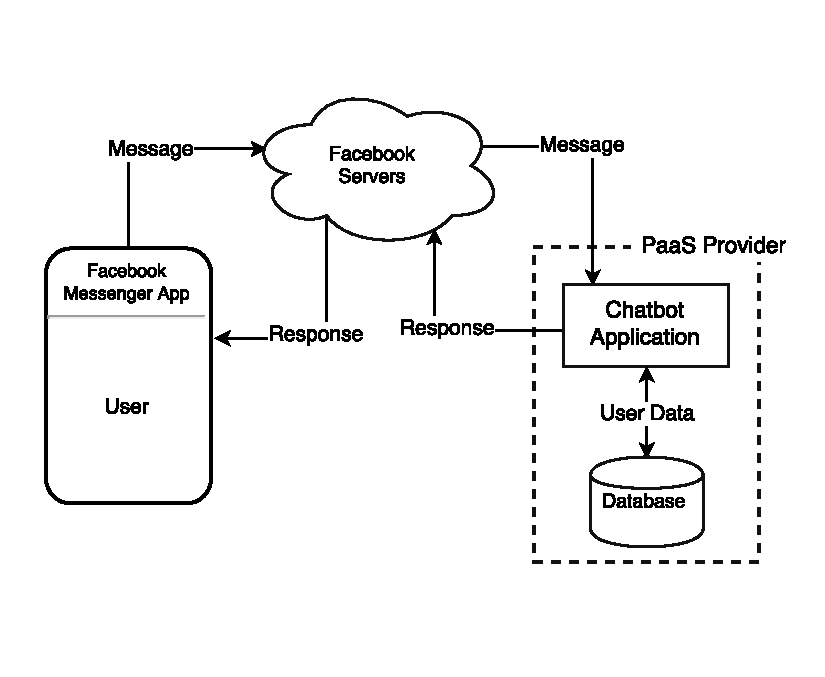
\includegraphics[width=5.1in]{../resources/diagrams/chatbot-component-overview.pdf}
    \caption{Prototype Component Overview}
    \label{fig:prototype_component_overview}
\end{figure}

\subsection{Deployment}

Language consideration, nodejs, java, other types, talk about heroku, hosting provider. Hosting provider.
Database provider discussion, integration, airtable,

\subsection*{Detailed Overview}

\begin{figure}[H]
    \centering
    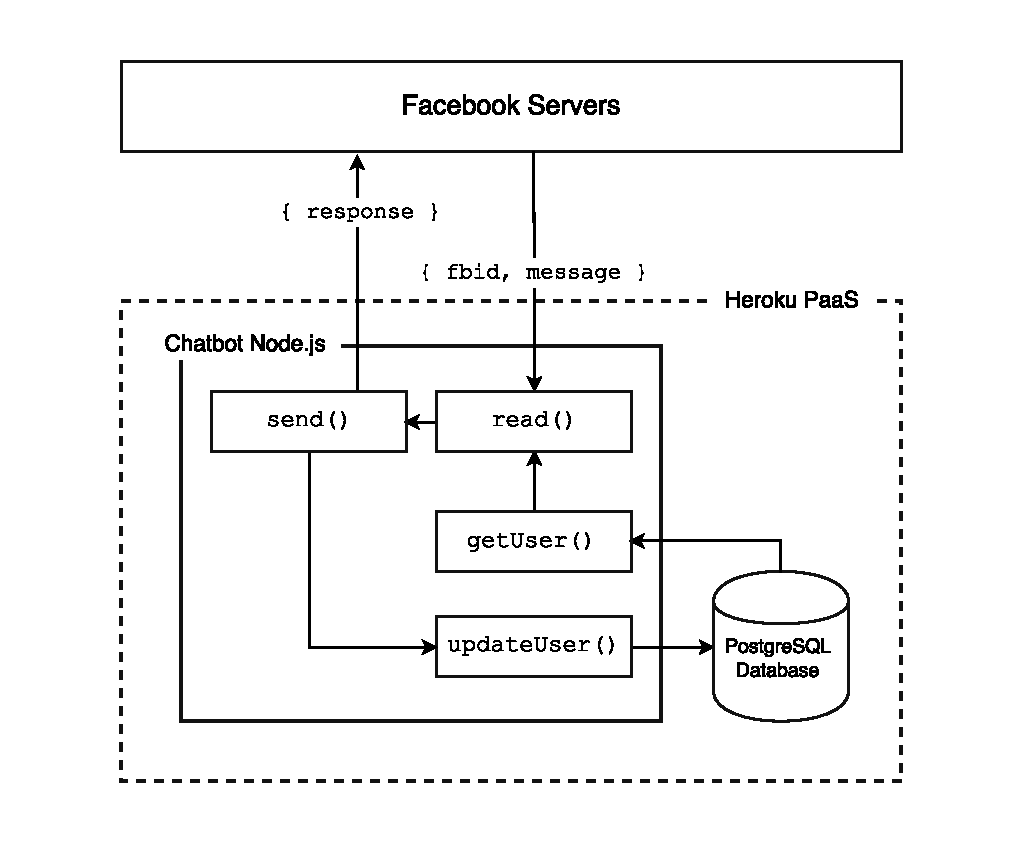
\includegraphics[width=6in]{../resources/diagrams/chatbot-detailed-overview.pdf}
    \caption{Detailed Overview}
    \label{fig:prototype_detailed_overview}
\end{figure}

Scalable architecture because heroku\newline

Implementaiton limitations about timezone with the scheduler\newline
Scheduler\newline
Free text input issues\newline

\subsection*{Technical Issues}
(Go through all meetings and list implementation issues here.)

Throughout the implementation process different techniques were explored to implement the design.
Some of the research areas were not used in the final prototype due to technical issues and limitations with the approach.

(TODO insert vibration screenshot here!)

Using vibration as a modality would've been a great additional modality to use.
Unfortunately the chatbot sandbox meant that the vibration ability in the phone could not be used, so another device would be used in combination with the bot.
Smart watches and fitness trackers were researched to test if they could programatically vibrate, with the pattern of vibration matching the frequency of the audio.
However, the majority of these devices did not have an API that exposed the vibration element. The best method was found to programatically set an alarm 1-minute into the future using a Fitbit fitness tracker.
This would trigger the vibration when the alarm sounded.
Although this would mean a 1-minute delay after completing a habit, a good user flow could've reduced the wait time with some additional dialogue.
But, this approach relied on the fitness tracker to sync with the phone after the alarm was programatically set. Unfortunately forcing the tracker to sync wasn't available, so this modality was abandoned.\newline
\newline
Another issue occured with stopping the audio after it had been played during a reward. If a user closed the reward box, there was no way to stop the audio, unless a user waited until it had finished. This limitation was very minor, but also showed how difficult it is to seemly connect a webview and a bot.


\subsection{Testing}

Test harness, tested the full functionality programatically. Hooking into Travis CI and other continuous integration services.
A pilot trial tested the basic chatbot functionality. Preparing for the full evaluation trails.


Several systems were reviewed to test their feasibility as a prototype. A chatbot was implemented as it can easily send notifications, has a short development time, high availability with cross-platform and is simple, with the user interface (UI) already built for us. The rise of social media and increasing use of humorous memes was utilised to provide the motivating content of the rewards (see figure~\ref{fig:setup}. This works well with the prototype integration into an existing social media messaging platform, \textit{Facebook Messenger} (\url{www.messenger.com}). Next we evaluate our hypotheses using our prototype with a study.
\newpage